\chapter{Tools and Techniques}

While it is difficult to identify specific patterns across all lethal sets $A_0$ under the $r$-neighbor bootstrap process, there are certain structures that appear frequently enough to warrant discussion. In this chapter, we examine such structures. We also introduce the following shorthand notation, which will appear throughout the remainder of this thesis. 

\begin{defn}
\label{defn:thickness}
Let $a_1, \dots, a_d$ be integers such that $a_1 \geq \dots \geq a_d \geq 1$. We define $G(a_1, \dots, a_d)$ to be the grid graph $\prod_{i=1}^d [a_i]$. Furthermore, we refer to the smallest value $a_d$ as the \emph{thickness} of $G(a_1, \dots, a_d)$.
\end{defn}
%We remark that $G(a_1, \dots, a_d)$ admits an optimal lethal set if and only if all other tuples obtained by permuting the values $a_1, \dots, a_d$ admit optimal lethal sets.
% We remark that this notation is the same as that used for the coordinates of a vertex, and make explicit note of this distinction when necessary. 

\section{The $d$-walls lemma}

We begin with the following lemma, which articulates more clearly the notion of a lethal set ``spanning" a grid (as we saw in Figure \ref{fig:two_infections}).

\begin{lem}
\label{lem:walls}
Let $A_0$ be an infected set on $G = \prod_{i=1}^d [a_i]$. Let $\overline{A_0} = V(G) \setminus A_0$, and let $H = G[\overline{A_0}]$ be the subgraph of $G$ induced by $\overline{A_0}$. For $1 \leq k \leq a_j$, let $F_{j,k} = \prod_{i=1}^{j-1} [a_i] \times \{k\} \times \prod_{i=j+1}^{d} [a_i]$ be the $k$th plane of $G$ in the $j$th dimension. If $H$ does not contain a path between $F_{j,1}$ and $F_{j,a_j}$, for all $1 \leq j \leq d$, then $A_0$ is lethal on $G$ under $d$-neighbor percolation.
\end{lem}

\begin{proof}
We proceed by induction on $|V(H)| = \prod_{i=1}^d a_i - |A_0|$. If $|V(H)| = 0$, then all vertices of $G$ are infected and we are done. Suppose $|V(H)| > 0$, and consider a connected component $Y$ of $H$. By hypothesis, for all $j \in [d]$, either $V(Y) \cap F_{j,1} = \emptyset$ or $V(Y) \cap F_{j,a_j} = \emptyset$ (or both). Suppose, without loss of generality, that $V(Y) \cap F_{j,a_j} = \emptyset$.
%Since $V(H) > 0$, there exists a $k_j < a_j$ such that $V(Y) \cap F_{j,k_j}$ is non-empty. 
For each $j \in [d]$, let $x_j$ be the maximum value such that $V(Y) \cap F_{j,x_j}$ is non-empty. Note that such an $x_j$ must exist since $|V(H)| > 0$. 

Consider the vertex $\vec{x} = (x_1, \dots, x_d) \in V(Y)$, and observe that 
$$\left\{\bigcup_{j \in [d]} F_{j,x_j+1}\right\} \cap  V(Y) = \emptyset.$$
In particular, note that $(x_1+1, x_2, \dots, x_d), \dots, (x_1, \dots, x_d+1) \in N_S(\vec{x})$. Therefore, $\vec{x}$ becomes infected. Furthermore, since $|V(H) \setminus \{\vec{x}\}| < |V(H)|$, the resulting graph percolates by induction. This completes the proof.
\end{proof}

\begin{cor}
\label{cor:walls}
Let $G$ be the grid graph $\prod_{i=1}^d [a_i]$. For each $j \in [d]$ and some $1 \leq k \leq a_j$, let 
$$M = \bigcup_{j,k} F_{j,k}$$
be a subset of the vertices of $G$ formed by the union of mutually orthogonal planes. If a set $A_0$ is lethal on $M$, then it is lethal on $G$. 
%Let $G$ be the grid graph $(a,b,c)$. If a set $A$ is lethal on three mutually orthogonal faces of $G$, then $A$ is lethal on $G$.
\end{cor}

\begin{proof}
Since $A_0$ is lethal on $M$, there exists a time $t$ where $M \subseteq A_t$. Therefore, for all $j \in [d]$, the graph $G[\overline{A_t}]$ cannot contain a path between $F_{j,1}$ and $F_{j,a_j}$. By Lemma \ref{lem:walls}, $A_0$ is lethal on $G$. 
%Let $X, Y, Z$ be three mutually orthogonal faces of $G$. By hypothesis, $X \cup Y \cup Z \subseteq A_t$ for some time $t$. Therefore, the graph $H = G[\overline{A_t}]$ cannot contain a path between vertices on orthogonal faces of $G$. By lemma \ref{lem:walls}, $G$ percolates.
\end{proof}

Corollary \ref{cor:walls} provides a cleaner characterization of certain lethal sets on $d$-dimensional grids in terms of their $(d-1)$-dimensional planes, provided these planes are mutually orthogonal. Here, we return to the notion first introduced in Chapter 1 of the capacity of a lethal set to span a grid. In particular, we see that the set in Figure \ref{fig:two_infections_a} is comprised of lethal sets under the 2-neighbor bootstrap process on the two one-dimensional orthogonal planes $F_{1,1}$ and $F_{2,1}$ of $[10]^2$. In this regard, the problem of obtaining perfect $d$-neighbor lethal sets on $d$-dimensional grids is reduced to the problem of determining a ``good" union $M$ of mutually orthogonal $(d-1)$-dimensional planes. 
%Once found, each face in $M$ can itself be infected by this same recursive process. 
In Chapter 7, we apply this idea to obtain an infinite family of three-dimensional grids from three orthogonal two-dimensional planes. However, we caution that the challenge of determining a ``good" union $M$ is non-trivial in general.

%(taken as a particular instance of Corollary \ref{cor:walls})
The following corollaries will be useful in our discussion of lethal sets on three-dimensional grids $G(a_1,a_2,a_3)$. 

\begin{cor}
\label{cor:three_walls_simple}
Let $G$ be the grid graph $G(a_1,a_2,a_3)$. If a set $A_0$ is lethal on $F_{1,i} \cup F_{2,j} \cup F_{3,k}$, for $i \in \{1,a_1\}$, $j \in \{1,a_2\}$, $k \in \{1,a_3\}$, then $A_0$ is lethal on $G$.
\end{cor}

\begin{proof}
By hypothesis, $A_0$ is lethal on $F_{1,i} \cup F_{2,j} \cup F_{3,k}$. Therefore, there exists some time $t$ for which $F_{1,i} \cup F_{2,j} \cup F_{3,k} \subseteq A_t$, and so $G[\overline{A_t}]$ satisfies the conditions of Lemma \ref{lem:walls}. We conclude that $A_0$ is lethal on $G$.
\end{proof}

\begin{cor}
\label{cor:three_walls}
Let $G$ be the grid graph $G(b_1,b_2,b_3)$. Let $b_1 = a_{1,1} + \dots + a_{1,k_1}$, $b_2 = a_{2,1} + \dots + a_{2,k_2}$, and $b_3 = a_{3,1} + \dots + a_{3,k_3}$. For $i \in [k_1]$ $($and $j \in [k_2]$, $\ell \in [k_3]$$)$, define $a_{1,0} = \emptyset$ $($resp. $a_{2,0}$ and $a_{3,0}$$)$ and let $S_{1,i} = [a_{1,i}] \setminus [a_{1,i-1}] \cup \{a_{1,i-1}\}$ $($resp. $S_{2,j}$ and $S_{3,\ell}$$)$. Let $G_{i,j,\ell}$ be the grid graph with vertex set
$$V(G_{i,j,\ell}) = S_{1,i} \times S_{2,j} \times S_{3,\ell}$$
and edges between adjacent vertices in each of the six cardinal directions. If each $G_{i,j,\ell}$ admits a lethal set $A_{i,j,\ell}$ on three orthogonal faces, then $A_0 = \cup A_{i,j,\ell}$ is lethal on $G$.
\end{cor}

\begin{proof}
Observe that $V(G) = \cup V(G_{i,j,\ell})$, for $i \in [k_1]$, $j \in [k_2]$ and $\ell \in [k_3]$. By Corollary \ref{cor:three_walls_simple}, each $G_{i,j,\ell}$ admits a lethal set. Therefore, all vertices of $G$ must become infected, and so $A_0$ is lethal on $G$.
\end{proof}

In the case of three-dimensional grids, it is instructive to think of the union of perpendicular faces $M$ over all $G_{i,j,\ell}$ as an unfolded surface. An illustration of this for $G(a_1,a_2,a_3)$ is shown in Figure \ref{fig:manifold_types}. We refer to $M$ as a manifold of $G$, and to this unfolded surface as a \emph{proper unfolding} of $M$. In Chapter 6, we examine other manifolds and their proper unfoldings. 

Since, by Corollary \ref{cor:walls}, any lethal set on $M$ is also lethal on $G$, it is often easier to identify lethal sets by examining these flattened unfolded structures. In fact, in the particular case of $M = F_{1,1} \cup F_{2,1} \cup F_{3,1}$, the surface area bound on $G(a_1,a_2,a_3)$ can be written in terms of the surface area bounds on flat, two-dimensional grids.

\begin{figure}[]
\centering
\hspace*{\fill}
\begin{subfigure}[b]{0.22\textwidth}
	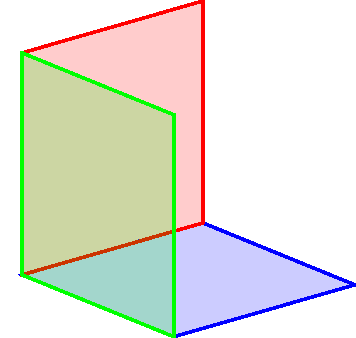
\includegraphics[width=\textwidth]{figures/3/manifold_a.pdf}
	\label{fig:manifold_a}
\end{subfigure} \hfill
\begin{subfigure}[b]{0.35\textwidth}
	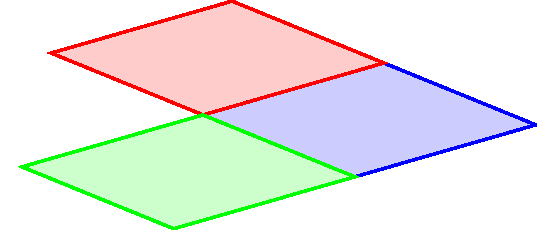
\includegraphics[width=\textwidth]{figures/3/manifold_flat.pdf}
	\label{fig:manifold_b}
\end{subfigure}
\hspace*{\fill}
\caption{Three perpendicular faces of $G(a_1,a_2,a_3)$ (left) and their representation as a flat unfolded surface (right).}
\label{fig:manifold_types}
\end{figure} 

\begin{lem}
\label{lem:unfolded_cube}
For $a_1 \geq a_2 \geq a_3 \geq 1$, 
$$\text{SA}(a_1, a_2, a_3) = \text{SA}(a_1+a_3-1, a_2+a_3-1, 1) - \text{SA}(a_3-1, a_3-1, 1).$$
\end{lem}

\begin{proof}
Taking the surface area bound on the righthand side of the above equation, we obtain
$$\text{SA}(a_1+a_3-1, a_2+a_3-1, 1) = \frac{a_1a_2 + a_1a_3 + a_2a_3 + a_3^2 -1}{3}$$
and
$$\text{SA}(a_3-1, a_3-1, 1) = \frac{a_3^2 -1}{3}.$$
Adding these two expressions together gives
$$\frac{a_1a_2 + a_1a_3 + a_2a_3}{3},$$
which is precisely the surface area bound for $G(a_1, a_2, a_3)$. 
\end{proof}

In the context of Figure \ref{fig:manifold_types}, this lemma tells us that a percolating set on the $G(a_1,a_2,a_3)$ grid (left of Figure \ref{fig:manifold_types}) is precisely the same size as a percolating set on the complete flattened rectangle minus the size of a percolating set on the missing region (right of Figure \ref{fig:manifold_types}). In practice, this lemma allows us to leverage an understanding of lethal sets on two-dimensional grids to obtain lethal sets in three dimensions. However, care is required in this process, as the region excluded from the two-dimensional unfolding must contain precisely the same number of infected vertices as the surface area bound.
%and the existence of an optimal set on a two-dimensional grid does not immediately guarantee the existence of such a set in three dimensions. 

\section{3-neighbor percolation on two-dimensional grids}

The above discussion suggests that an understanding of the behavior of 3-neighbor percolation on two-dimensional grids is of use in our investigation of 3-neighbor percolation on $G(a_1,a_2,a_3)$ grids. In Chapter 5 we examine the problem of 3-neighbor percolation on square two-dimensional grids, and answer a question posed by Benevides, Bermond, Lesfari and Nisse regarding the value of $m([n]^2, 3)$. Here, we describe some of the structural properties of lethal sets on two-dimensional grids that will prove useful in that analysis. The following propositions are due to Benevides et al \cite{benevides:2021}. 

\begin{prop}
\label{prop:corners}
Let $A_0$ be a lethal set on $[a_1] \times [a_2]$ under 3-neighbor percolation. Then $A_0$ contains all four corner vertices of $[a_1] \times [a_2]$.
\end{prop}

\begin{proof}
Since corner vertices in $[a_1] \times [a_2]$ have degree 2, they cannot become infected. Therefore, since $A_0$ is lethal, it must contain all corner vertices.
\end{proof}

\begin{prop}
\label{prop:border}
Let $B$ be the set of vertices on the border of $[a_1] \times [a_2]$, and let $u,v \in B$ be adjacent vertices. If $A_0$ is a lethal set under 3-neighbor percolation, then $A_0 \cap \{u,v\} \neq \emptyset$.
\end{prop}

\begin{proof}
Assume for contradiction that $A_0 \cap \{u,v\} = \emptyset$. By Proposition \ref{prop:corners}, neither $u$ nor $v$ is a corner vertex. Since $u,v$ are border vertices, $d(u) = d(v) = 3$. Because $A_0$ is lethal, $u$ and $v$ must become infected. Suppose, without loss of generality, that $u$ is infected first. This is impossible, since $d(u) = 3$ and $v$ is not infected.
\end{proof}

\begin{prop}
\label{prop:immune_regions}
Let $A_0$ be a lethal set on $[a_1] \times [a_2]$ under 3-neighbor percolation. Let $H = V([a_1] \times [a_2]) \setminus A_0$. Then the subgraph induced by $H$ is acyclic and each component of $H$ contains at most one border vertex.
\end{prop}

\begin{proof}
Suppose for contradiction that $C$ is a cycle in $H$. Let $v \in C$ be the first vertex of $C$ to become infected. Note that $v$ has two uninfected neighbors in $C$. Since $d(v) \leq 4$, $v$ cannot become infected, a contradiction.

Suppose $P$ is a path in $H$ with endpoints on the border. No vertex $v$ in $P$ can become infected, since $v$ has at most two neighbors outside of $P$.
\end{proof}

\begin{table}[]
\centering
\begin{subfigure}{0.3\textwidth}
	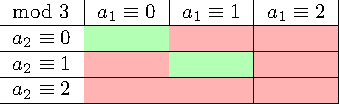
\includegraphics[width=\textwidth]{tables/1/integral_bounds_thickness_1.pdf}
	\caption{$a_3 \equiv 1 \pmod 3$}
	\label{tab:integral_bounds_a}
\end{subfigure} \hfill%
\begin{subfigure}{0.3\textwidth}
	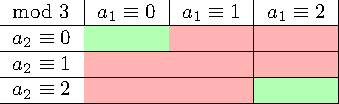
\includegraphics[width=\textwidth]{tables/1/integral_bounds_thickness_2.pdf}
	\caption{$a_3 \equiv 2 \pmod 3$}
	\label{tab:integral_bounds_b}
\end{subfigure} \hfill%
\begin{subfigure}{0.3\textwidth}
	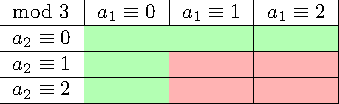
\includegraphics[width=\textwidth]{tables/1/integral_bounds_thickness_3.pdf}
	\caption{$a_3 \equiv 0 \pmod 3$}
	\label{tab:integral_bounds_c}
\end{subfigure}
\caption{Integrality of grids by congruence class. Green indicates integral surface area bound.}
\label{tab:integral_bounds}
\end{table} 

Proposition \ref{prop:immune_regions} more clearly articulates the notion of immune regions discussed in Chapter 1. While such immune regions exist in higher-dimensional grids, their structure is substantially harder to characterize. 

It will be insightful to consider the surface area bound on two-dimensional grids in the context of Propositions \ref{prop:corners}, \ref{prop:border} and \ref{prop:immune_regions}. For simplicity, we introduce the following terms. We refer to grids with integral surface area bounds as \emph{divisibility cases} and grids with non-integral bounds as \emph{non-divisibility cases}. The divisibility and non-divisibility cases for three-dimensional grids where $r=3$ are illustrated in Table \ref{tab:integral_bounds}. We refer to the lethal set $A_0 \subseteq V(G)$ in $G(a_1,a_2,a_3)$ that matches the surface area bound as \emph{optimal}. Furthermore, if $G(a_1,a_2,a_3)$ is a divisibility case, we call $A_0$ \emph{perfect}. For brevity, if $G(a_1,a_2,a_3)$ admits an optimal lethal set, we refer to the tuple $(a_1,a_2,a_3)$ as \emph{optimal}, and if $G(a_1,a_2,a_3)$ admits a perfect lethal set, we refer to the tuple $(a_1,a_2,a_3)$ as \emph{perfect}. We remark that any tuple $(a_1, a_2, a_3)$ is optimal if and only if all other tuples obtained by permuting the values $a_1, a_2, a_3$ are optimal.

Recall from Chapter 1 that a lethal initial infection $A_0$ is perfect if it contains no adjacent vertices, and if all vertices $v \in A_{0}$, $t > 0$, are infected by precisely $d$ neighbors. Therefore, by Propositions \ref{prop:corners} and \ref{prop:border}, if  $[a_1] \times [a_2]$ admits a perfect lethal set, then $a_1, a_2 \equiv 1 \pmod 2$. Furthermore, every component of the subgraph $H$ induced by uninfected vertices must contain exactly one border vertex (otherwise the second condition on perfect infections would be violated). In Chapter 6, we use these observations to prove that the only two-dimensional grids that admit perfect lethal sets under 3-neighbor bootstrap percolation are of the form $[2^n-1]^2$.

\begin{figure}[]
\centering
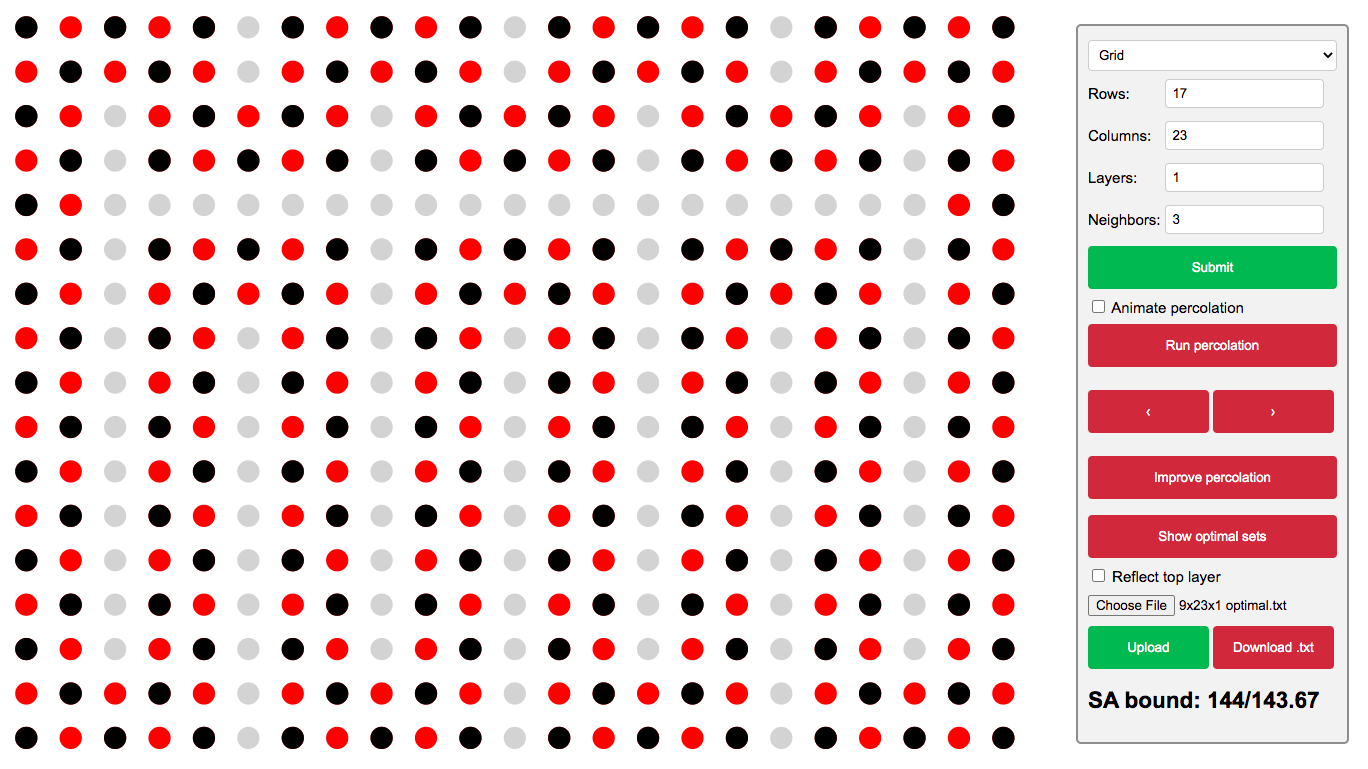
\includegraphics[width=\textwidth]{figures/2/visualizer}
\caption{The visualization tool with a infected set.}
\label{fig:visualizer}
\end{figure} 

\section{Visualizer}

In addition to the conceptual tools presented above, many of the results in this thesis were obtained with the help of a visualization tool. This resource allows a user to experimentally infect vertices in two- and three-dimensional grids, and observe the step-by-step $r$-neighbor percolation process. As far as we are aware, such a tool did not previously exist for the problem of bootstrap percolation. In this section, we provide an overview of the functionality of this resource (which we refer to as the \emph{visualizer}), and highlight features that could prove useful in further research. The visualizer is located at \texttt{https://ahblay.pythonanywhere.com}, and the reader is encouraged to examine the lethal sets presented in later chapters as they appear (although this is not necessary to understand the results).

\subsection{Control panel}

%e.g. they wish to examine the grid $[17] \times [23]$ under 3-neighbor percolation, and so select ``Grid" from the dropdown menu and choose 17 rows, 23 columns, 1 layer, and a threshold of 3 neighbors) This renders a grid of gray vertices. The user then selects those vertices that they wish to infect and, when satisfied, clicks ``Run percolation." This allows the user to step through the phases of infection

The basic functionality of the visualizer allows a user to enter the parameters of their problem, select a set of initially infected vertices, and step through the percolation process by time-step. These options are made available to the user in a control panel, shown on the righthand side of Figure \ref{fig:visualizer}. The control panel features the following:
\begin{itemize}
\item A dropdown menu to choose between percolation on a grid, and percolation on a torus;
\item Text boxes to enter the size of the grid (resp. torus);
\item A text box to enter the threshold number of neighbors to spawn an infection;
\item A submit button, which renders the chosen parameters as a grid of clickable gray circles;
\item Buttons to initiate and step through the percolation process, and a checkbox to animate it;
\item A button labeled ``Improve percolation," which removes unnecessary infections (should they exist);
\item An option to select from a list of existing lethal sets;
\item A checkbox to reflect infected vertices;
\item Buttons to upload/download an infected set as a text file.
\end{itemize}
We highlight the design and representation of grids as matrices of clickable vertices, the choice between grid and torus, the ``Improve percolation" button, the ability to view existing lethal sets as well as upload/download them, and the option to reflect the pattern of infected vertices. 

One of the challenges of visualizing the problem of bootstrap percolation arises from the fact that many grids are large and high-dimensional. This is perhaps the greatest limitation of the visualizer. The current iteration of the tool renders vertices as clickable regions in an HTML \texttt{canvas} element, which does not respond well to re-scaling. As a result, large grids contain very small vertices, which complicates the process of selecting an initial infection. Furthermore, \texttt{canvas} does not natively support 3-dimensional structures, and so 3-dimensional grids are simply rendered as a stack of their 2-dimensional layers. 

Users are able to select between percolation on a grid, and percolation on a torus. This choice does not impact the representation of the grid (resp. torus). However, when stepping through the phases of infection, vertices at the top of the grid are treated as neighbors of those on the bottom, and similarly for left and right. 

In this chapter (and in Chapter 6) we saw (shall see) that certain patterns of infected vertices are always lethal. The fickleness of bootstrap percolation regularly precludes us from simply copying these patterns across all grids to obtain perfect lethal sets. However, sometimes these patterns can be augmented with additional infections. If a set $A_0$ is lethal and above the surface area bound, the ``Improve percolation" button attempts to remove non-essential infections. It does this by removing a random vertex $v$ from $A_0$ and checking if the resulting set is lethal. If it is, the new infection $A_0 \setminus \{v\}$ is rendered on the screen. 

In pursuit of determining new perfect lethal sets, it is often helpful to examine and alter existing ones. Whenever a user clicks ``Run percolation" on a perfect lethal set, a text file containing the lethal configuration of vertices is stored in a database. This file is made accessible to all future users through the ``Show optimal sets" window. We hope that ongoing use of this tool will passively allow for the accumulation of a number of lethal sets in 2- and 3-dimensions. In addition to accessing known lethal sets via the ``Show optimal sets" button, users are able to upload sets from a local text file. These files must be configured as a sequence of X's and O's, with rows on new lines, and layers separated by a blank line. An example of this format can be obtained by creating an infected grid on the visualizer and selecting ``Download .txt". 

The ``Reflect top layer" checkbox is another resource designed to increase the efficiency of experimentally generating lethal sets. We have found in our research that certain grids, especially of the form $[a_1] \times [a_2] \times [2]$, have symmetric infections in their top and bottom layers. By choosing ``Reflect top layer", these symmetries are generated automatically. 

%\subsection{Design}

\subsection{Improvements}

The visualization tool was developed primarily as a means to engage with the structure of lethal sets directly. Initially, it was intended as a private tool to help discern the often complex patterns in these sets. For this reason, it contains a number of quirks and bugs that were either treated as features, or ignored and never resolved. In this section, we discuss some of these issues and suggest possible improvements to make the tool useful to a broader audience. 

The most significant bug occurs when a user attempts to alter an infected set during the percolation process. This bug is a direct consequence of the manner in which 

% ability to toggle between the three different configurations of a set
As we discussed in the prior section, one limitation of HTML \texttt{canvas} elements is the inability to conveniently represent three dimensional objects. We circumvented this issue by representing grids as a sequence of two-dimensional layers. While this strategy is effective, it limits a user's ability to clearly identify patterns that appear between these layers. Through experimentation, we found that toggling between different orientations of the grid allowed us to discover patterns that were otherwise hidden. In the current version of the visualizer, there is no convenient way to obtain different orientations of a grid. We propose an additional button that cycles through the $d$ orientations of a grid. This feature would likely be simple to implement, and yield substantial results.

% ability to infect vertices by clicking and dragging
We also discussed the challenge of clicking on vertices in large grids, due to the inability to effectively zoom in on the \texttt{canvas} element. While the best solution to this problem likely requires a complete overhaul of the representation of the grid (using some other front-end library designed to better represent and interact with grid-like structures), an intermediate and simpler possibility is to improve the manner in which vertices are selected. In particular, we propose a change that allows sequences of vertices to be simultaneously selected by clicking and dragging. This should be fairly easy to implement, as one can track the \texttt{mouseDown} event in Javascript, and keep a list of the vertices that the cursor touches during this time.  

% highlight cells that experience infection from >r neighbors
% improving the manner in which sets are improved (this is a computational problem)
When attempting to construct a lethal set, it is often the case that one begins with a particular configuration of vertices, and makes small changes to accommodate the particular parity or congruence class of the grid. One existing resource to aid in this process is the ``Improve percolation" button. In its current state, this button is only able to remove unnecessary vertices from already lethal sets. However, it would we useful if it could also augment existing sets in such a way that they become more infectious. This could take the form of either adding vertices to infectious sets that are below the surface area bound, or changing the position of existing infections to increase the infectiousness of the initial set. 

In a similar vein, recall that non-integral sets $A_0$ contain vertices that experience infection from more than $r$ neighbors. If the size of $A_0$ is well above the surface area bound, the location of such vertices can provide a good indication of where improvements in the structure of $A_0$ are likely to be found. One possible implementation could be to highlight vertices that do not realize their ``infectious potential". 

% nice presentation of existing lethal sets in the database
From a cosmetic perspective, the presentation of existing perfect lethal sets is currently difficult to parse and should be improved. We suggest that these files be arranged by the number of layers in the grid. Additionally, there is currently no capacity to represent and store constructions that apply to large families of grids. We currently provide large example files that clearly exhibit a repeating pattern. However, this choice is both less convenient and less convincing. 

% increase the efficiency of the percolation algorithm

% count the number of timesteps

% randomize initial infections

% higher dimensions (could be HARD)

% make the visualization tool into a puzzle game???

% COMMENT
% COMMENT
% COMMENT
% COMMENT
% COMMENT
% COMMENT

\begin{comment}

\section{Outline of main result}

%As discussed in Chapter 1, the surface area bound is not always integral. We refer to grids with integral surface area bounds as \emph{divisibility cases} and grids with non-integral bounds as \emph{non-divisibility cases}. The divisibility and non-divisibility cases for three-dimensional grids where $r=3$ are illustrated in Table \ref{tab:integral_bounds}. Let $A_0 \subseteq V(G)$ be a lethal set on $G$ that matches the surface area bound. We call $A_0$ \emph{perfect} if $G$ is a divisibility case, and \emph{optimal} if $G$ is a non-divisibility case. 

The proof of Theorem \ref{thm:main_result} relies on the existence of a number of infinite families of perfect lethal sets. These are constructions that match the surface area bound and can be extended in one or two dimensions. Tables \ref{tab:integral_bounds_2}, \ref{tab:integral_bounds_3} and \ref{tab:integral_bounds_5} display these families. Proofs of the lethality of these constructions are presented in Chapter 7 and Appendix A. 

In the following chapter, we present a technique for recursively assembling small perfect sets into large perfect sets. By repeatedly applying this recursion to the sets illustrated in Tables \ref{tab:integral_bounds_2}, \ref{tab:integral_bounds_3} and \ref{tab:integral_bounds_5}, we are able to obtain perfect sets for all grids $G(a_1, a_2, a_3)$ where $a_1 \geq a_2 \geq a_3 \geq 5$. We extend this result to non-divisibility cases by applying the recursion to a small set of optimal grids illustrated in Appendix A. 

\begin{table}[]
\centering
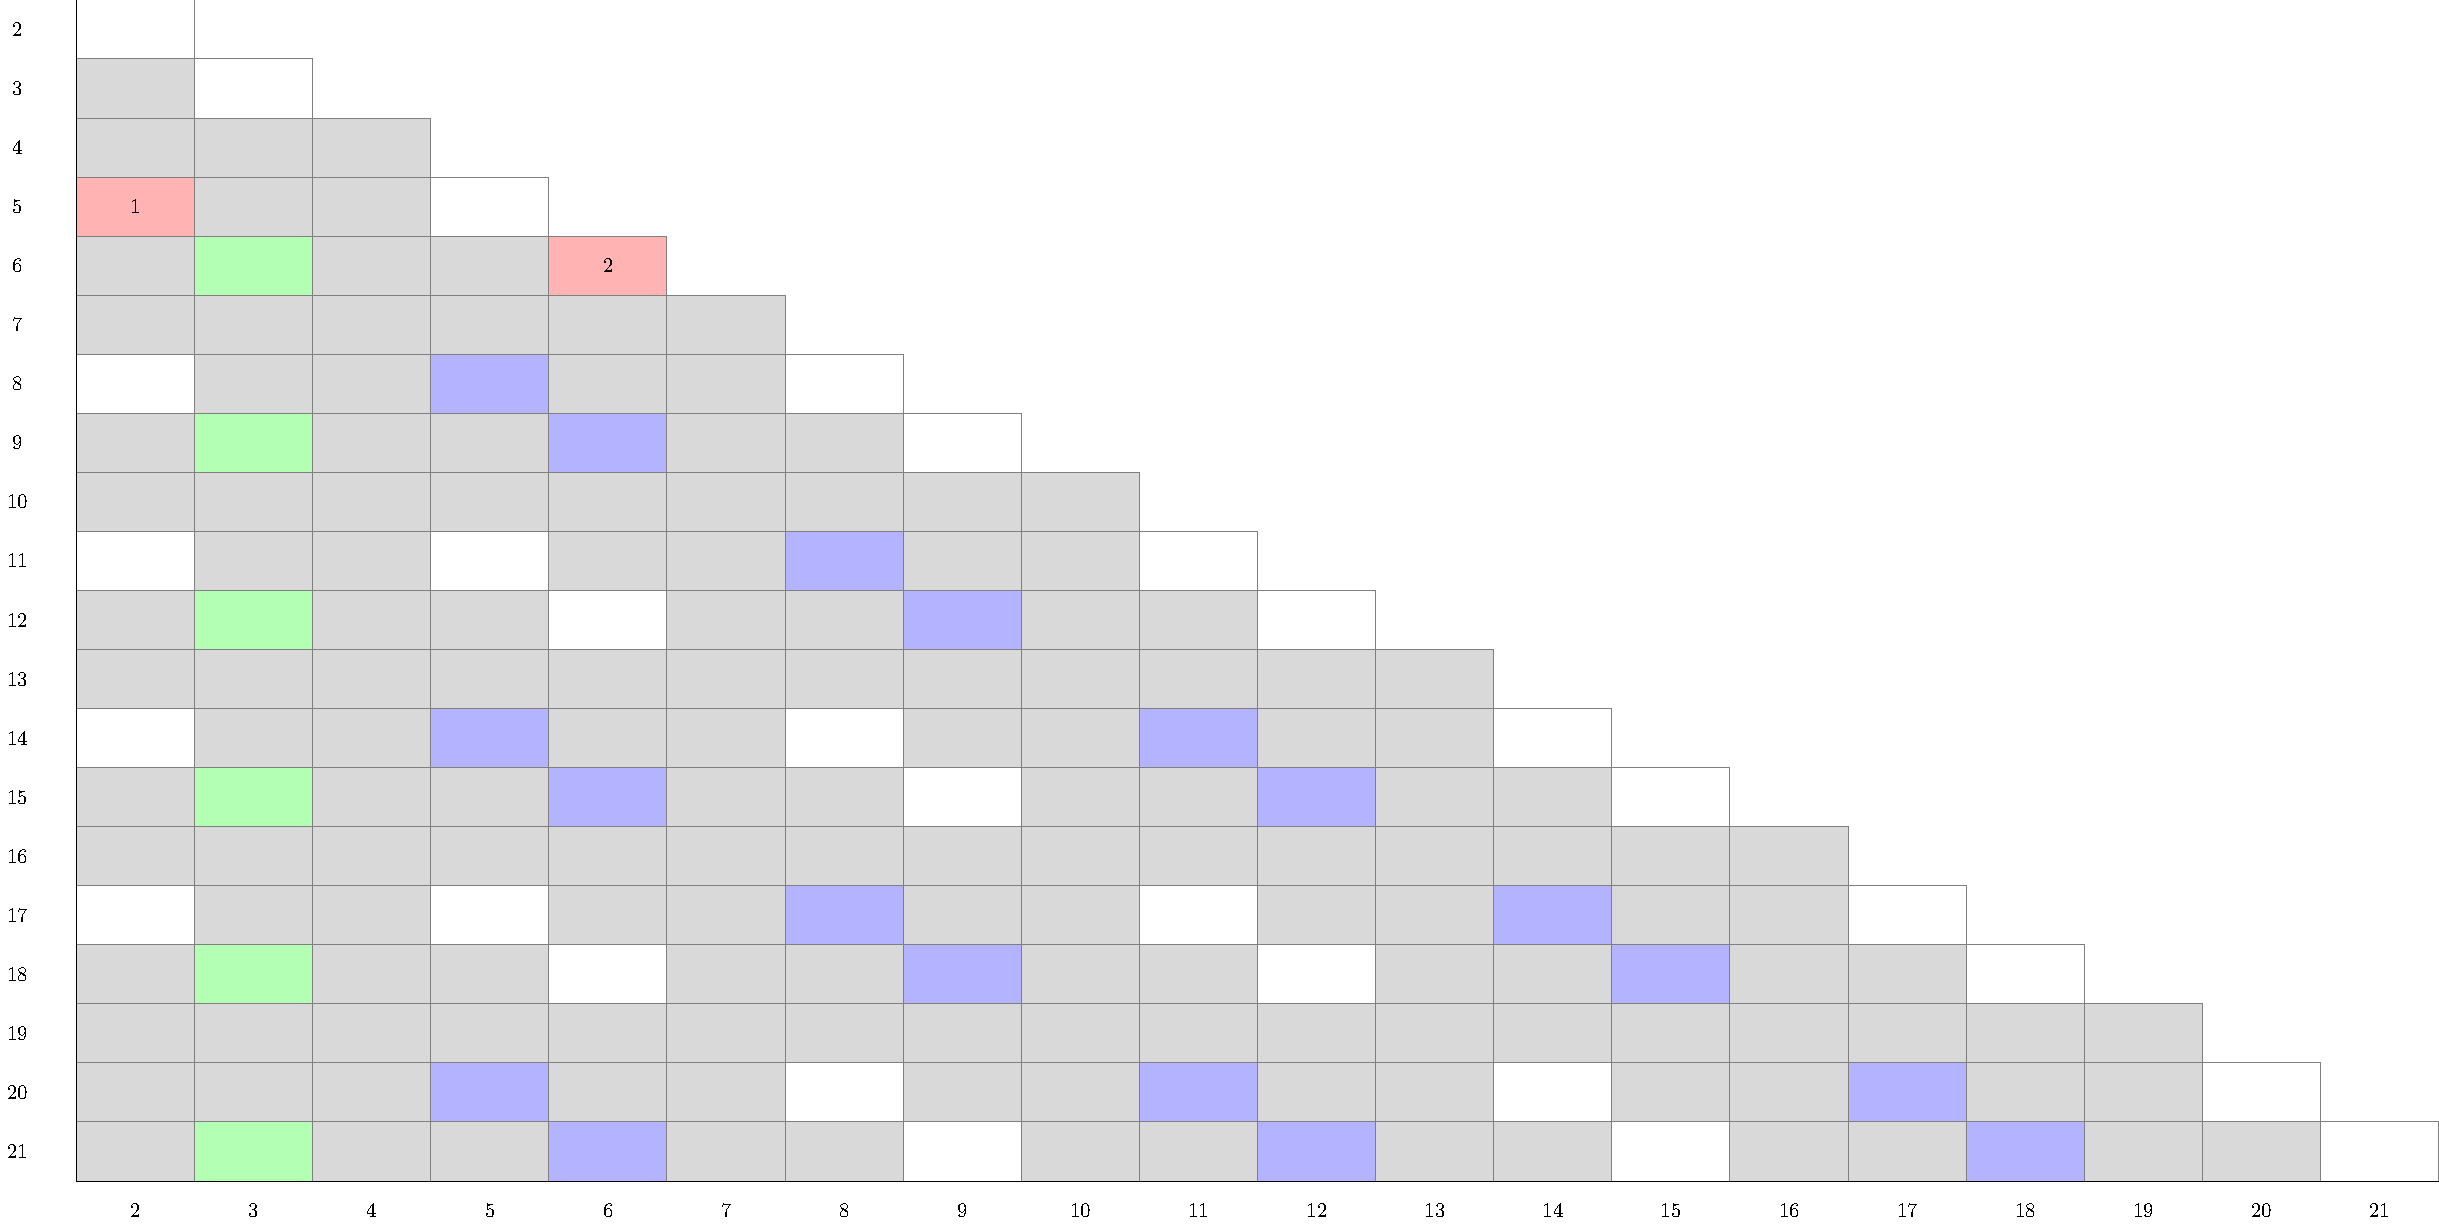
\includegraphics[width=\textwidth]{tables/2/thickness_2.pdf}
\caption{Thickness 2 constructions used in the proof of Theorem \ref{thm:main_result}. Blue and green cells represent infinite families of constructions. Red cells are individual constructions. Divisibility cases are white and non-divisibility cases are gray.}
\label{tab:integral_bounds_2}
\end{table} 

\begin{table}[]
\centering
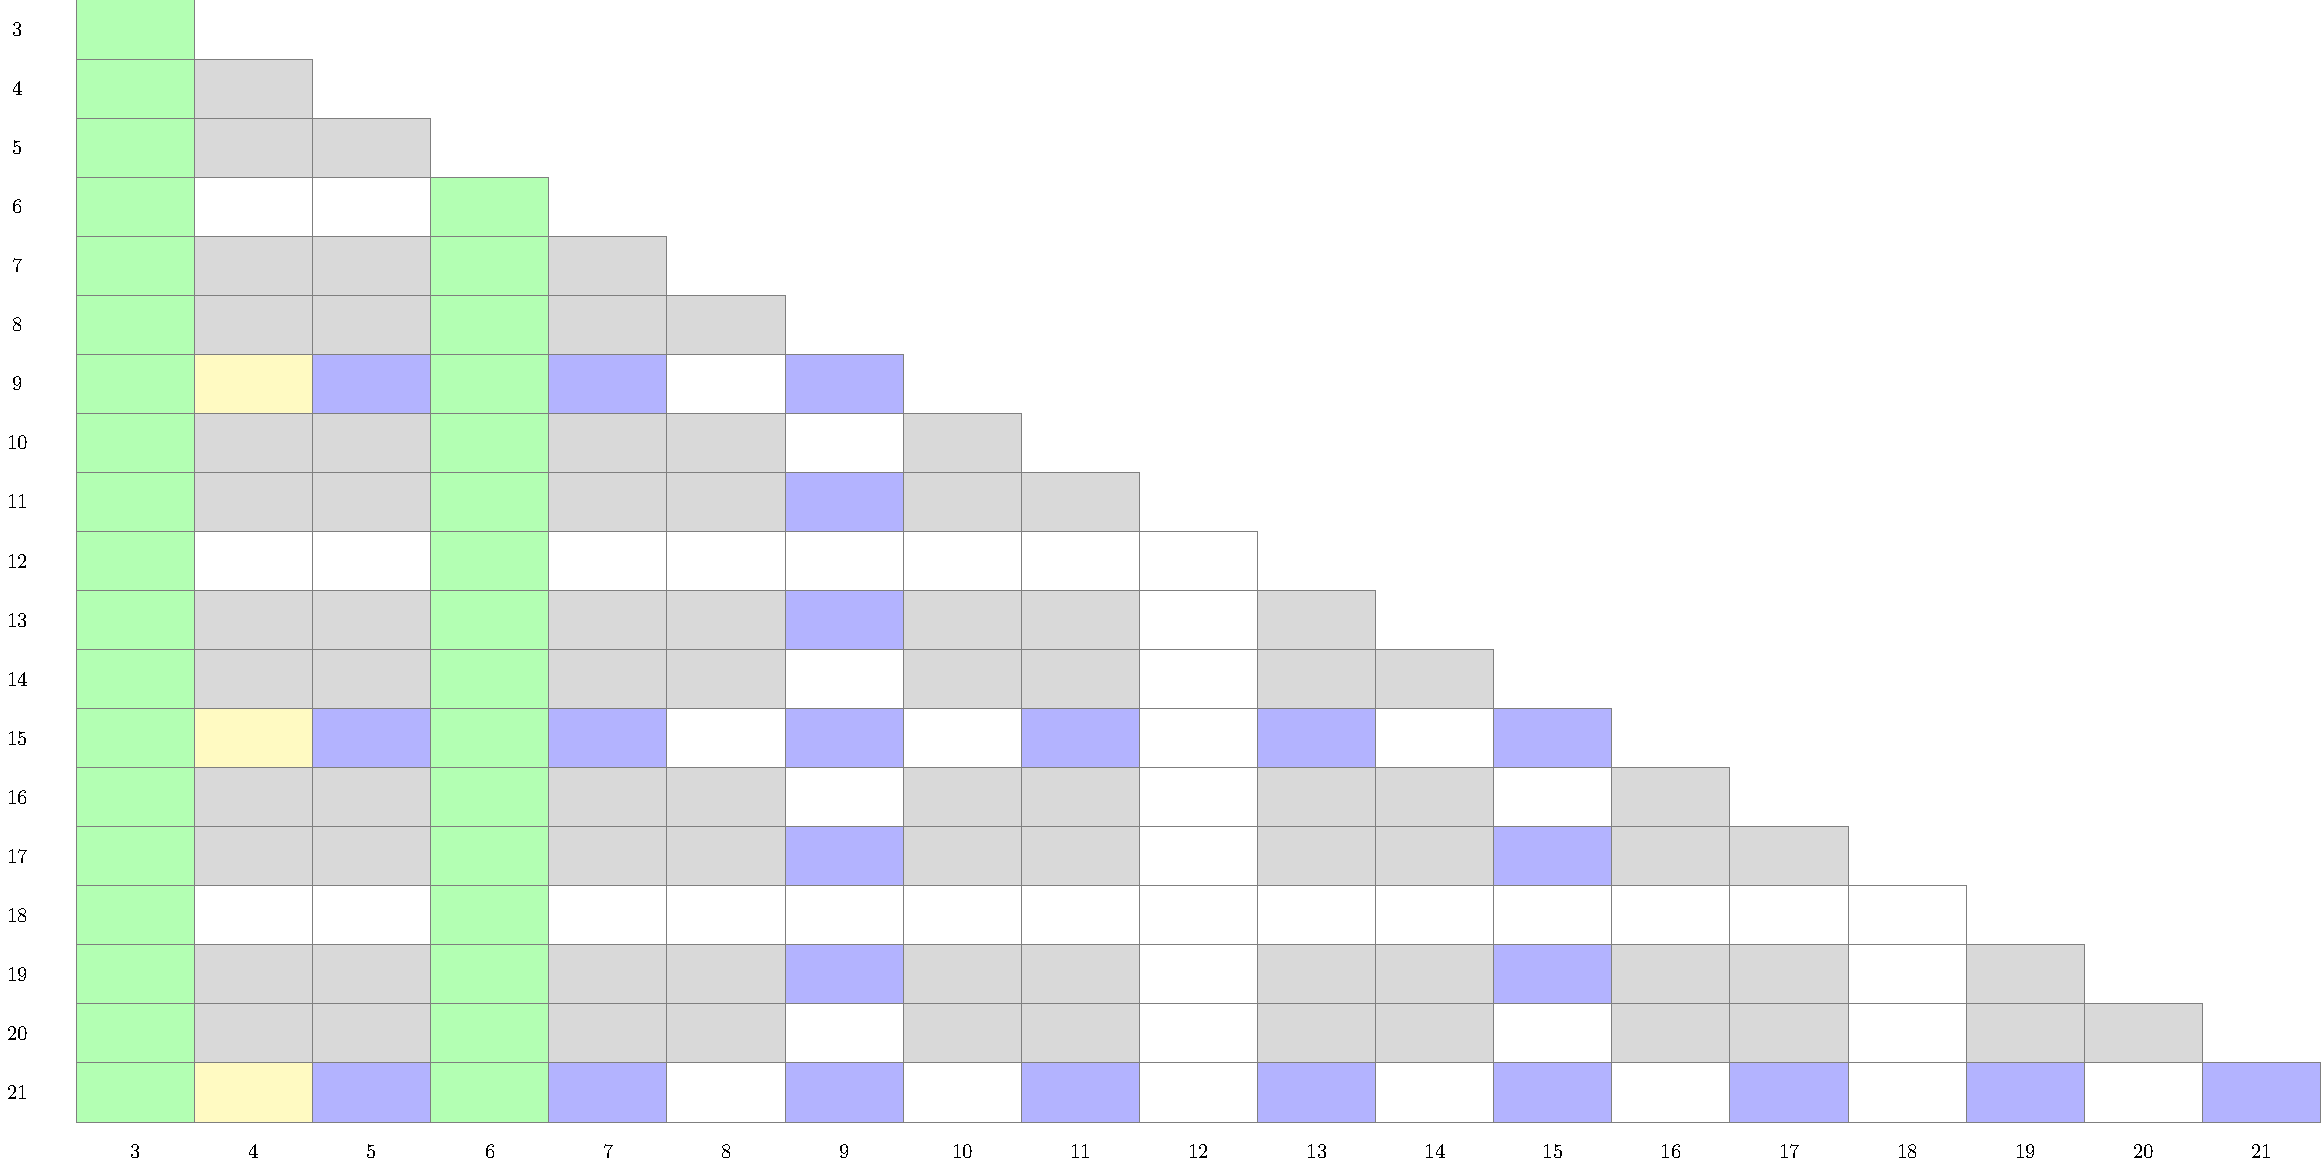
\includegraphics[width=\textwidth]{tables/2/thickness_3.pdf}
\caption{Thickness 3 constructions used in the proof of Theorem \ref{thm:main_result}. Blue, green and yellow cells represent infinite families of constructions. Red cells are individual constructions. Divisibility cases are white and non-divisibility cases are gray.}
\label{tab:integral_bounds_3}
\end{table} 

\begin{table}[]
\centering
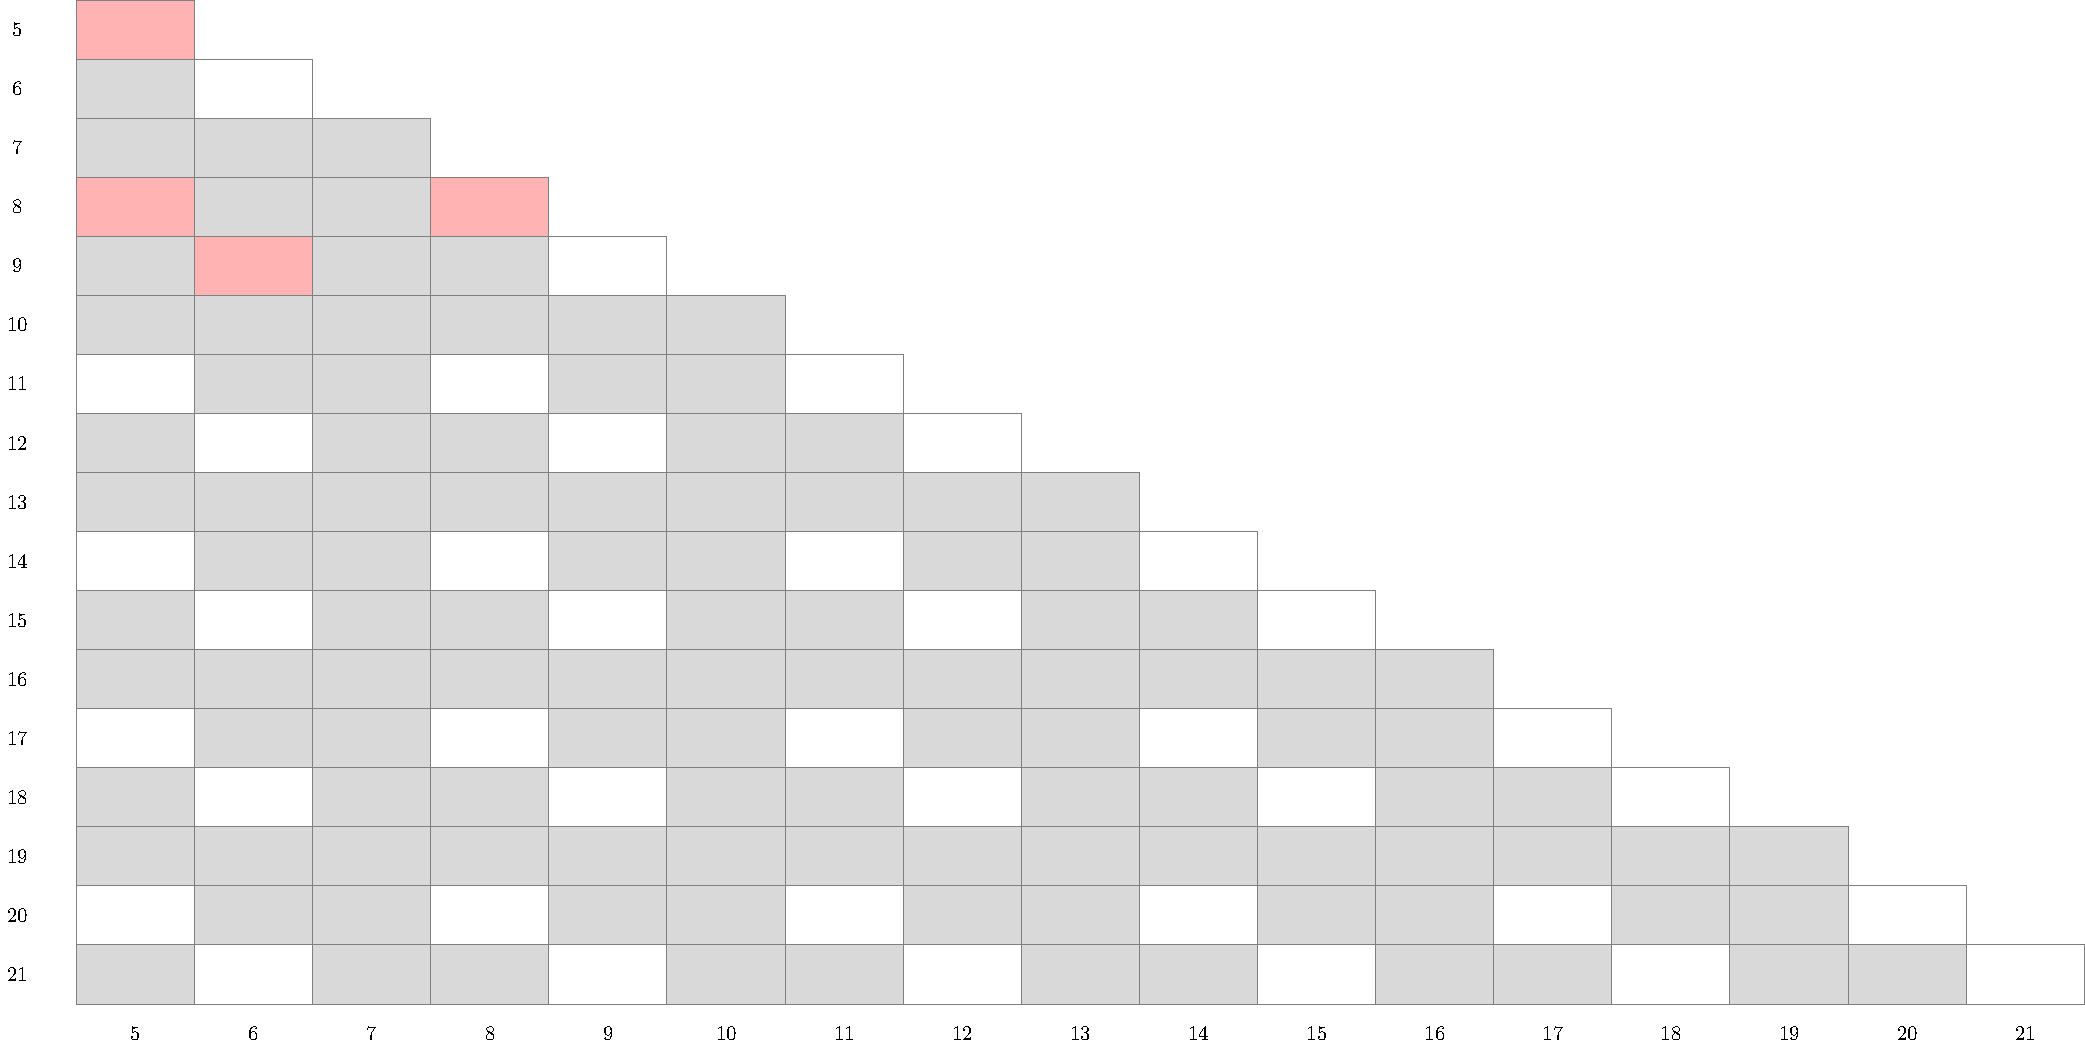
\includegraphics[width=\textwidth]{tables/2/thickness_5.pdf}
\caption{Thickness 5 constructions used in the proof of Theorem \ref{thm:main_result}. Red cells are individual constructions. Divisibility cases are white and non-divisibility cases are gray.}
\label{tab:integral_bounds_5}
\end{table}

\section{Manifolds}

We refer to unions $M$ of perpendicular faces as manifolds. As suggested in the previous section, there are a wide variety of possible manifold structures for a given grid. We highlight two particular structures in Figure \ref{fig:manifold_types}. The following two lemmas show that it is possible to obtain perfect lethal sets on these structures from existing perfect sets on grids of thickness one. 

%As discussed above, the capacity to generate ``good" sets $M$ is critical for building perfect lethal sets recursively. QUESTION: If we apply the above recursive process to faces, do the bounds match up? We shall examine the particular case of orthogonal faces on three-dimensional grids.

% I KNOW THIS ISN'T QUITE RIGHT. 
% The idea is that the three faces minus their pairwise intersections, plus their complete intersection matches the lower bound on (a,b,c)
\begin{lem}
\label{lem:manifold_a}
Let $G$ be the grid graph $(a_1,a_2,a_3)$ and 
$$M = F_{1,1} \triangle F_{2,1} \triangle F_{3,1}.$$
Note that $G[M]$ is isomorphic to the disjoint union of grids $(a_1 -1, a_2 -1, 1), (a_2 -1, a_3 -1, 1), (a_3 -1, a_1 -1, 1)$. Let $S_{1,2}, S_{2,3}, S_{3,1}$ be perfect lethal sets under 3-neighbor percolation on each of these grids, respectively. Let $S$ be the set of vertices $S_{1,2} \cup S_{2,3} \cup S_{3,1}$ under isomorphism from $(a_1 -1, a_2 -1, 1) \cup (a_2 -1, a_3 -1, 1) \cup (a_3 -1, a_1 -1, 1)$ to $G[H]$. Then $S \cup (1,1,1)$ is lethal and perfect on $G$.
%Note that $F_{j,k}$ is isomorphic to $\prod_{i \in [d], i \neq j} [a_i]$. If a set $S$ is lethal and perfect on each of $[a_1-1] \times [a_2-1], [a_2-1] \times [a_3-1], [a_3-1] \times [a_1-1]$ under 3-neighbor percolation, then $S \cup (0,0,0)$ is lethal on $G$. 
\end{lem}

\begin{proof}
This proof is just algebra. Assume that each of the three faces has a lethal set at the surface area bound, add them all up, and observe that the resulting sum is precisely the surface area bound on the grid, minus one point. 
\end{proof}

WHOOPS! THE FOLLOWING PROOF DOESN'T QUITE WORK. SHOULD ADD 4/3 OF A POINT, NOT 2 POINTS.

\begin{lem}
\label{lem:manifold_b}
Let $G$ be the grid graph $(a_1,a_2,a_3)$ and let $M$ be the symmetric difference of vertex sets on the red, green and blue faces illustrated in Figure \ref{fig:manifold_b}. Let $S$ be a perfect lethal set under 3-neighbor percolation on $G[M]$. Then $S \cup \{\text{ opposite corners of the green face }\}$ is perfect and lethal on $G$.
\end{lem}

\begin{proof}
A bunch of basic algebra shows that the bound match up. The two points on the green face are sufficient to guarantee the lethality of $S$ on the entire manifold. 
\end{proof}

QUESTION: Does this extend to $d$-neighbor percolation on $d$-dimensional grids?

QUESTION: The above lemma applies to the circumstance where $M$ is half of the surface area of $G$. What if $M$ is a different set of mutually orthogonal faces? How do we write this is general, where none of the faces lie on the surface of the grid?

QUESTION: What is the relationship between that case (mentioned above) and the block recursion? 

%Consider the symmetric difference of orthogonal faces, and let $S$ be a lethal set on this structure. 
%We can use the above lemma in conjunction with the block recursion. In particular, each block is lethal on 

\begin{figure}[]
\centering
\begin{subfigure}{0.45\textwidth}
	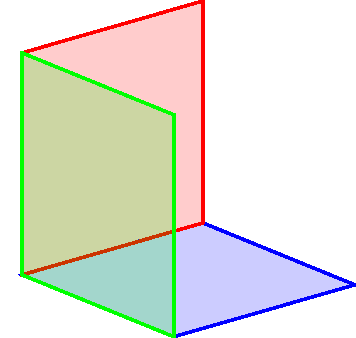
\includegraphics[width=\textwidth]{figures/3/manifold_a.pdf}
	\caption{Three perpendicular walls.}
	\label{fig:manifold_a}
\end{subfigure} \hfill%
\begin{subfigure}{0.45\textwidth}
	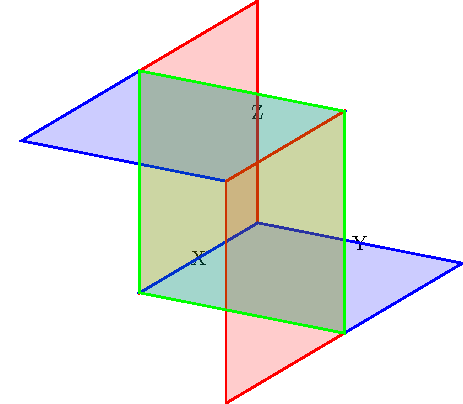
\includegraphics[width=\textwidth]{figures/3/manifold_b.pdf}
	\caption{Five perpendicular walls.}
	\label{fig:manifold_b}
\end{subfigure}
\caption{Two types of manifold used in our constructions.}
\label{fig:manifold_types}
\end{figure} 

%The set $M$, obtained from the union of mutually orthogonal faces of $G$, 
It bears mention that many lethal sets on manifolds are discovered through trial and error. One strategy is to imagine these manifolds as folded pieces of paper, and to identify lethal sets on their unfolded nets. This technique is discussed in more detail in Chapter \{CONSTRUCTIONS\}. 

\subsection{Integrality of bounds}

Not all grids have integral surface area bounds. We refer to such grids as \emph{non-divisibility cases}. The non-divisibility cases for three-dimensional grids where $r=3$ are illustrated in red in Table \ref{tab:integral_bounds}. 

As discussed in Chapter 1, percolation in non-divisible grids is inefficient in one of two ways: either $A_0$ contains adjacent vertices, or at some time-step $i$, there exists a vertex $v \in V \setminus A_i$ such that $N_{A_i}(v) > r$. 
% In the first case, the inefficiency is a consequence of two adjacent vertices in $A_0$; heuristically, we may view this as poor distribution of infection across the grid. In the second case, the inefficiency results from excessive infection in a particular region; a vertex is over-exposed. 

It is insightful to consider this behavior in the context of Theorem \ref{thm:torus_lb}. Instead of thinking of $m_{IH}$ at the number of edges between $I$ and $H$, we shall consider it to represent the perimeter, or surface area, of the initial infection $I$. 
%In particular, the existence of adjacent vertices in $A_0$ corresponds precisely to inequality in $m_{IH} \leq 2d|I| - 2(ab+bc+ca)$, where $2(ab+bc+ca)$ is the surface area of the grid. 
%In these cases, we are guaranteed the existence of at least one cell that is infected by more than $r$ neighbors. This is a direct consequence of the surface area argument; since the final surface area of infection is non-integral and surface area is non-increasing

\subsection{A different characterization}

We shall find it useful to think about the problem of bootstrap percolation in terms of the graph induced by the set of uninfected vertices $V \setminus A_i$ at some time-step $t_i$. 

\subsection{Attributes of $G[V \setminus A]$}

No cycles, no paths between opposite faces. Reference to Benevides.

\subsection{The lower bound}

Let us reconsider the our proof of the lower bound in this new framework. 

\subsection{Surface area, optimality, trees, and components}

The surface area bound is not always integral. In cases where it is not, this sub-optimality can be traced to a particular time-step where an uninfected cell is infected by more than $r$ neighbors. The proof of the lower bound on the torus considers the number of components in $T[V \setminus A]$, as each such component necessarily collapses in on a vertex where this occurs. In the grid, this circumstance can be avoided by permitting components to abut the perimeter. What is the relationship here?

\subsection{The bipartition (and when to violate it)}

Discuss the heuristic of placing infections on one side of the bipartition and when this technique fails. 

\subsection{A potentially interesting proof framework}

A discussion on the broad structure of the proof of the lower bound on the torus as presented in Benevides. Note that this proof relies on a sequence of inequalities, and that two of these inequalities characterize precise conditions that are necessary for a set to be lethal. Discuss how the proof might change as a function of the dimension of the grid. 

\end{comment}
